%%%%%%%%%%%%%%%%%%%%%%%%%%%%%%%%%%%%%%%%%
% Wenneker Assignment
% LaTeX Template
% Version 2.0 (12/1/2019)
%
% This template originates from:
% http://www.LaTeXTemplates.com
%
% Authors:
% Vel (vel@LaTeXTemplates.com)
% Frits Wenneker
%
% License:
% CC BY-NC-SA 3.0 (http://creativecommons.org/licenses/by-nc-sa/3.0/)
% 
%%%%%%%%%%%%%%%%%%%%%%%%%%%%%%%%%%%%%%%%%

%----------------------------------------------------------------------------------------
%	PACKAGES AND OTHER DOCUMENT CONFIGURATIONS
%----------------------------------------------------------------------------------------

\documentclass[11pt]{scrartcl} % Font size

%%%%%%%%%%%%%%%%%%%%%%%%%%%%%%%%%%%%%%%%%
% Wenneker Assignment
% Structure Specification File
% Version 2.0 (12/1/2019)
%
% This template originates from:
% http://www.LaTeXTemplates.com
%
% Authors:
% Vel (vel@LaTeXTemplates.com)
% Frits Wenneker
%
% License:
% CC BY-NC-SA 3.0 (http://creativecommons.org/licenses/by-nc-sa/3.0/)
% 
%%%%%%%%%%%%%%%%%%%%%%%%%%%%%%%%%%%%%%%%%

%----------------------------------------------------------------------------------------
%	PACKAGES AND OTHER DOCUMENT CONFIGURATIONS
%----------------------------------------------------------------------------------------

\usepackage{amsmath, amsfonts, amsthm} % Math packages

\usepackage{listings} % Code listings, with syntax highlighting

\usepackage[english]{babel} % English language hyphenation

\usepackage{graphicx} % Required for inserting images
\graphicspath{{Figures/}{./}} % Specifies where to look for included images (trailing slash required)

\usepackage{booktabs} % Required for better horizontal rules in tables

\numberwithin{equation}{section} % Number equations within sections (i.e. 1.1, 1.2, 2.1, 2.2 instead of 1, 2, 3, 4)
\numberwithin{figure}{section} % Number figures within sections (i.e. 1.1, 1.2, 2.1, 2.2 instead of 1, 2, 3, 4)
\numberwithin{table}{section} % Number tables within sections (i.e. 1.1, 1.2, 2.1, 2.2 instead of 1, 2, 3, 4)

\setlength\parindent{0pt} % Removes all indentation from paragraphs

\usepackage{enumitem} % Required for list customisation
\setlist{noitemsep} % No spacing between list items

%----------------------------------------------------------------------------------------
%	DOCUMENT MARGINS
%----------------------------------------------------------------------------------------

\usepackage{geometry} % Required for adjusting page dimensions and margins

\geometry{
	paper=a4paper, % Paper size, change to letterpaper for US letter size
	top=2.5cm, % Top margin
	bottom=3cm, % Bottom margin
	left=3cm, % Left margin
	right=3cm, % Right margin
	headheight=0.75cm, % Header height
	footskip=1.5cm, % Space from the bottom margin to the baseline of the footer
	headsep=0.75cm, % Space from the top margin to the baseline of the header
	%showframe, % Uncomment to show how the type block is set on the page
}

%----------------------------------------------------------------------------------------
%	FONTS
%----------------------------------------------------------------------------------------

\usepackage[utf8]{inputenc} % Required for inputting international characters
\usepackage[T1]{fontenc} % Use 8-bit encoding

\usepackage{fourier} % Use the Adobe Utopia font for the document

%----------------------------------------------------------------------------------------
%	SECTION TITLES
%----------------------------------------------------------------------------------------

\usepackage{sectsty} % Allows customising section commands

\sectionfont{\vspace{6pt}\centering\normalfont\scshape} % \section{} styling
\subsectionfont{\normalfont\bfseries} % \subsection{} styling
\subsubsectionfont{\normalfont\itshape} % \subsubsection{} styling
\paragraphfont{\normalfont\scshape} % \paragraph{} styling

%----------------------------------------------------------------------------------------
%	HEADERS AND FOOTERS
%----------------------------------------------------------------------------------------

\usepackage{scrlayer-scrpage} % Required for customising headers and footers

\ohead*{} % Right header
\ihead*{} % Left header
\chead*{} % Centre header

\ofoot*{} % Right footer
\ifoot*{} % Left footer
\cfoot*{\pagemark} % Centre footer
 % Include the file specifying the document structure and custom commands

%----------------------------------------------------------------------------------------
%	TITLE SECTION
%----------------------------------------------------------------------------------------
\title{	
	\normalfont\normalsize
	\textsc{Universidad Central del Ecuador}

	\textsc{Facultad de Ingeniería y Ciencias Aplicadas}

	\textsc{Carrera de Ingeniería Informática}
	\vspace{6pt} % Whitespace
	\rule{\linewidth}{0.5pt}\\ % Thin top horizontal rule
	\vspace{20pt} % Whitespace
	{\huge Las Data Class y su uso en las Apps}\\ % The assignment title
	\vspace{12pt} % Whitespace
	\rule{\linewidth}{2pt}\\ % Thick bottom horizontal rule
	\vspace{12pt} % Whitespace
}

\author{\LARGE Nelson Ricardo Baquero} % Your name

\date{\normalsize\today} % Today's date (\today) or a custom date

\begin{document}

\maketitle % Print the title

%----------------------------------------------------------------------------------------
%	FIGURE EXAMPLE
%----------------------------------------------------------------------------------------

\section{¿Cuántos constructores puede tener una data class?}

Tiene un constructor principal donde se puede definir valores predeterminados para las variables.

\begin{lstlisting}
data class Person(val name: String, val age: Int)
\end{lstlisting}

Se pueden definir también constructores secundarios que tomen variables arbitrarias, con la condición que siempre deben delegarse al contructor principal.

\begin{lstlisting}
data class Person(val name: String) {
    constructor(name: String, age: Int) : this(name)
}
\end{lstlisting}

Además, si trabaja en un proyecto con compatibilidad con java, es posible especificar la anotación \textbf{@JvmOverloads} para generar varios constructores en bitecode que puedan ser utilizados por código Java.

\begin{lstlisting}
data class Person @JvmOverloads constructor(val name: String, 
                                            val age: Int? = 0)
\end{lstlisting}

%------------------------------------------------

\section{Numere las ventajas que tienen las data class sobre las clases regulares}

\begin{enumerate}
	\item Requiere escribir mucho menos código por parte del programador.
	\item Son inmutables, lo que significa que comprobar la igualidad en dos instancias con el mismo contenido siempre retornará \emph{verdadero}.
	\item Posee varias utilidades basadas en su contenido: equals(), toString(), componentN(), copy().
\end{enumerate}

\section{¿Cuáles son las limitaciones que tienen en la programación orientada a objetos?}

\begin{itemize}
	\item Las data classes no pueden ser marcadas como: abstract, sealed, open o inner.
	\item Los constructores de las data classes siempre deben recibir al menos un parámetro.
\end{itemize}

\section{¿Qué son las destructuring declarations y cómo funcionan?}

Las \emph{destructuring declarations} sirven para declarar múltiples variables al mismo tiempo. Es especialmente útil para ahorrar tiempo al escribir las declaraciones de variables que posee un objeto intermedio.

\begin{lstlisting}
val (name, age) = person
\end{lstlisting}

Ejemplo, retornar dos variables desde una función y utilizar una \emph{destructuring declaration}' para obtenerlas:

\begin{lstlisting}
data class Result(val result: Int, val status: Status)
fun function(...): Result {
    // codigo
    return Result(result, status)
}

// Para utilizar la funcion y destructurar el resultado:
val (result, status) = function(...)
\end{lstlisting}

\section{Cree una data class como ejemplo}

\begin{figure}[h] % [h] forces the figure to be output where it is defined in the code (it suppresses floating)
	\centering
	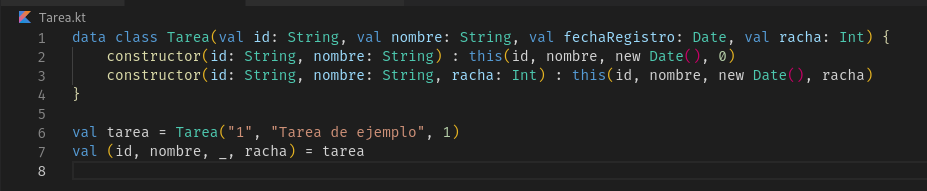
\includegraphics[width=\columnwidth]{data_class.png} % Example image
	\caption{Ejemplo de data class en Kotlin}
\end{figure}

\end{document}
